
\( C(x) = (5x - 2)\e^{-0{,}2x} + 2 \).

\subsection*{1.}

On lit une production d'environ 5{,}4 tonnes pour un coût maximal.

\subsection*{2.}

\paragraph{a.}
\begin{align*}
C'(x) &= C_m(x) \\
&= 5\e^{-0{,}2x} - 0{,}2 \times (5x - 2)\e^{-0{,}2x} \\
&= \e^{-0{,}2x}(5 - x + 0{,}4) \\
&= (-x + 5{,}4)\e^{-0{,}2x}.
\end{align*}

\paragraph{b.} Donc :
\[
-x + 5{,}4 < 0 \quad \text{si} \quad 5{,}4 < x \quad \text{ou} \quad x > 5{,}4.
\]

\paragraph{c.}

On sait que, quel que soit le réel \( x \), \( \e^{-0{,}2x} > 0 \), donc le signe de \( C_m(x) \) est celui de \( -x + 5{,}4 \).

D'après la question précédente \( C \) est croissante sur \( [0 \,;\, 5{,}4[ \), puis décroissante sur \( ]5{,}4 \,;\, 10] \), avec un maximum en :
\[
C(5{,}4) = (5 \times 5{,}4 - 2) \e^{-0{,}2 \times 5{,}4} + 2 \approx 10{,}4899.
\]

\begin{center}
\begin{tikzpicture}
\tkzTabInit[lgt=3.5, espcl=3]{$x$ / 1, {Signe de $C'(x)$} / 1, {$C(x)$} / 2}{${0}$, ${5{,}4}$, ${10}$}
\tkzTabLine{,+,0,-,}
\tkzTabVar{-/{$$},+/{$\approx 10{,}49$},-/{$$}}{/}
\end{tikzpicture}
\end{center}

\paragraph{d.}

Le coût total mensuel maximal sur l'intervalle considéré est donc environ de 10 490 €.

